\documentclass{beamer}

\usepackage[frenchb]{babel}
\usepackage[T1]{fontenc}
\usepackage[latin1]{inputenc}
\usepackage{hyperref}
\usepackage{listings}
\usepackage{fancyvrb}
\usepackage{tikz}
\usepackage{framed}
\usepackage{algorithm}
\usepackage{algorithmic}
\usetheme{Boadilla}
\usecolortheme{dolphin}

\lstnewenvironment{codeC}
{ \lstset{language=C,
    otherkeywords={printf,scan}}
}
{}
\newcommand{\red}{\textcolor{red}}
%\newcommand \emph
%Default size : 12.8 cm * 9.6 cm

\newenvironment<>{codeblock}[1]{%begin
  \setbeamercolor{block title}{fg=darkgray,bg=yellow}%
  \begin{block}{#1}}
  % \begin{codeC}}
  %  {\end{codeC}
{  
\end{block}}

\newenvironment<>{termblock}[1]{
    \setbeamercolor{block title}{fg=white,bg=lightgray}%
    \begin{block}{#1}}
%     \begin{Verbatim}}
{%\end{Verbatim}
\end{block}
}
%\newcommand{\output}[1]{

%%% Param�tres du cours (� r�gler)
%Num�ro du cours
\newcommand{\nb}{1}

\title[Cours n�\nb]{Cours n�\nb - Algorithmes et premiers pas en C}
\author[]{julien.brajard@upmc.fr}
\institute[Polytech' UPMC]{Polytech' UPMC}
\date{28 Septembre 2015}
\begin{document}
%%%%%%%%%%%%%%%%%%%%% SLIDES DE TITRE
\begin{frame}
\titlepage
\centering{
\url{http://australe.upmc.fr} (onglet EPU-C5-IGE Info Gen)}
\end{frame}
%%%%%%%%%%%%%%%%%%%%%
\begin{frame}
\frametitle{Plan du cours n�\nb}
\tableofcontents[hideallsubsections]
\end{frame}

%%%%%% SECTION 12

%%%%%%%%%%%%%%%%%%%%% SECTION 1
\section{Les algorithmes}\label{section:1}
\begin{frame}
  \begin{columns}
    \column{4.8cm}
    \tableofcontents[currentsection,hideothersubsections]
    \column{7cm}
    \centering{
      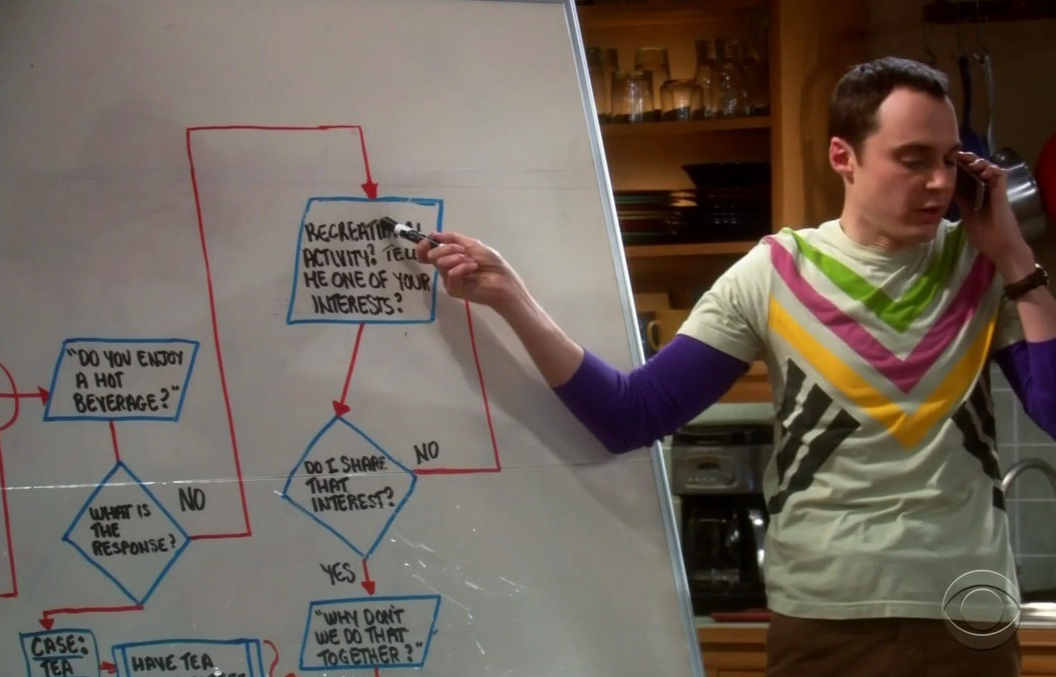
\includegraphics[width=7cm]{fig/Algorithm-sheldon.png}
      \textit{``I believe I've isolated the algorithm for making friends.''}
      \small{
        \hfill Sheldon Cooper, 
        \hfill in \textit{The Big Band Theory}, Season 2, Episode 13
      }
    }
  \end{columns}
  
\end{frame}

%%%%%%%%%%%%%%%%%%%%% 

\subsection{Introduction}
\begin{frame}
  \frametitle{Pourquoi faire appel � des algorithmes ?}
  Pour automatiser des t�ches
  
  Exemples :
  \begin{itemize}
  \item M�tier � tisser\\
  \item M�thode de calcul � la main d'une division\\
  \item Recette de cuisine\\
  \item ...\\
  \end{itemize}
\end{frame}

%%%%%%%%%%%%%%%%% 

\begin{frame}
  \frametitle{Qu'est-ce qu'un algorithme ?}
  \begin{alertblock}{D�finition}
    Un algorithme est un ensemble 
    ordonn� d'instructions simples
    permettant de r�soudre un probl�me.
  \end{alertblock}
\end{frame}

%%%%%%%%%%%%%%%%%% 

\begin{frame}
\frametitle{Remarques}
  \begin{block}{Un algorithme n�cessite :}
    \begin{itemize}
    \item Des objets sur lesquels travailler,\\
    \item Un langage non ambigu,\\
    \item Des sp�cifications (description de l'algorithme).\\
    \end{itemize}
  \end{block}
  
  \begin{block}{}
    Il n'existe g�n�ralement pas un unique algorithme pour traiter un probl�me.
  \end{block}
\end{frame}

%%%%%%%%%%%%%%%%%

\begin{frame}
  \frametitle{Historique}
  \begin{description}
\item[3�me si�cle avant JC] \textit{Livre VII des El�ments d'Euclide}
 \begin{columns}[T]
    \column{8cm}
D�termination du plus grand diviseur commun entre deux nombres :
PGCD(12,8)=4\\

 \column{4cm}
    \centering{
      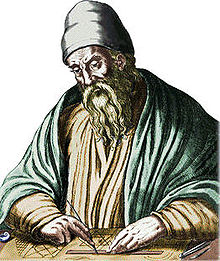
\includegraphics[width=4cm]{fig/Euclide.jpg}
}
\end{columns}
\item[8�me si�cle apr�s JC] \textbf{\textit{Al-Khawarizmi}} : M�thodes de r�solution d'�quations.
Son nom est � l'origine du mot "algorithme".
\end{description}
\end{frame}

%%%%%%%%%%%%%%%%%%%%%%%%%%%%%%%%%%%%%%%%%%%%%%%%%%%%%%%%%%%%%%%%%%%

\subsection{Construction d'un algorithme}

\begin{frame}
  \begin{columns}
    \column{4.8cm}
    \tableofcontents[currentsection,hideothersubsections,currentsubsection]
    \column{7cm}
    \centering{
      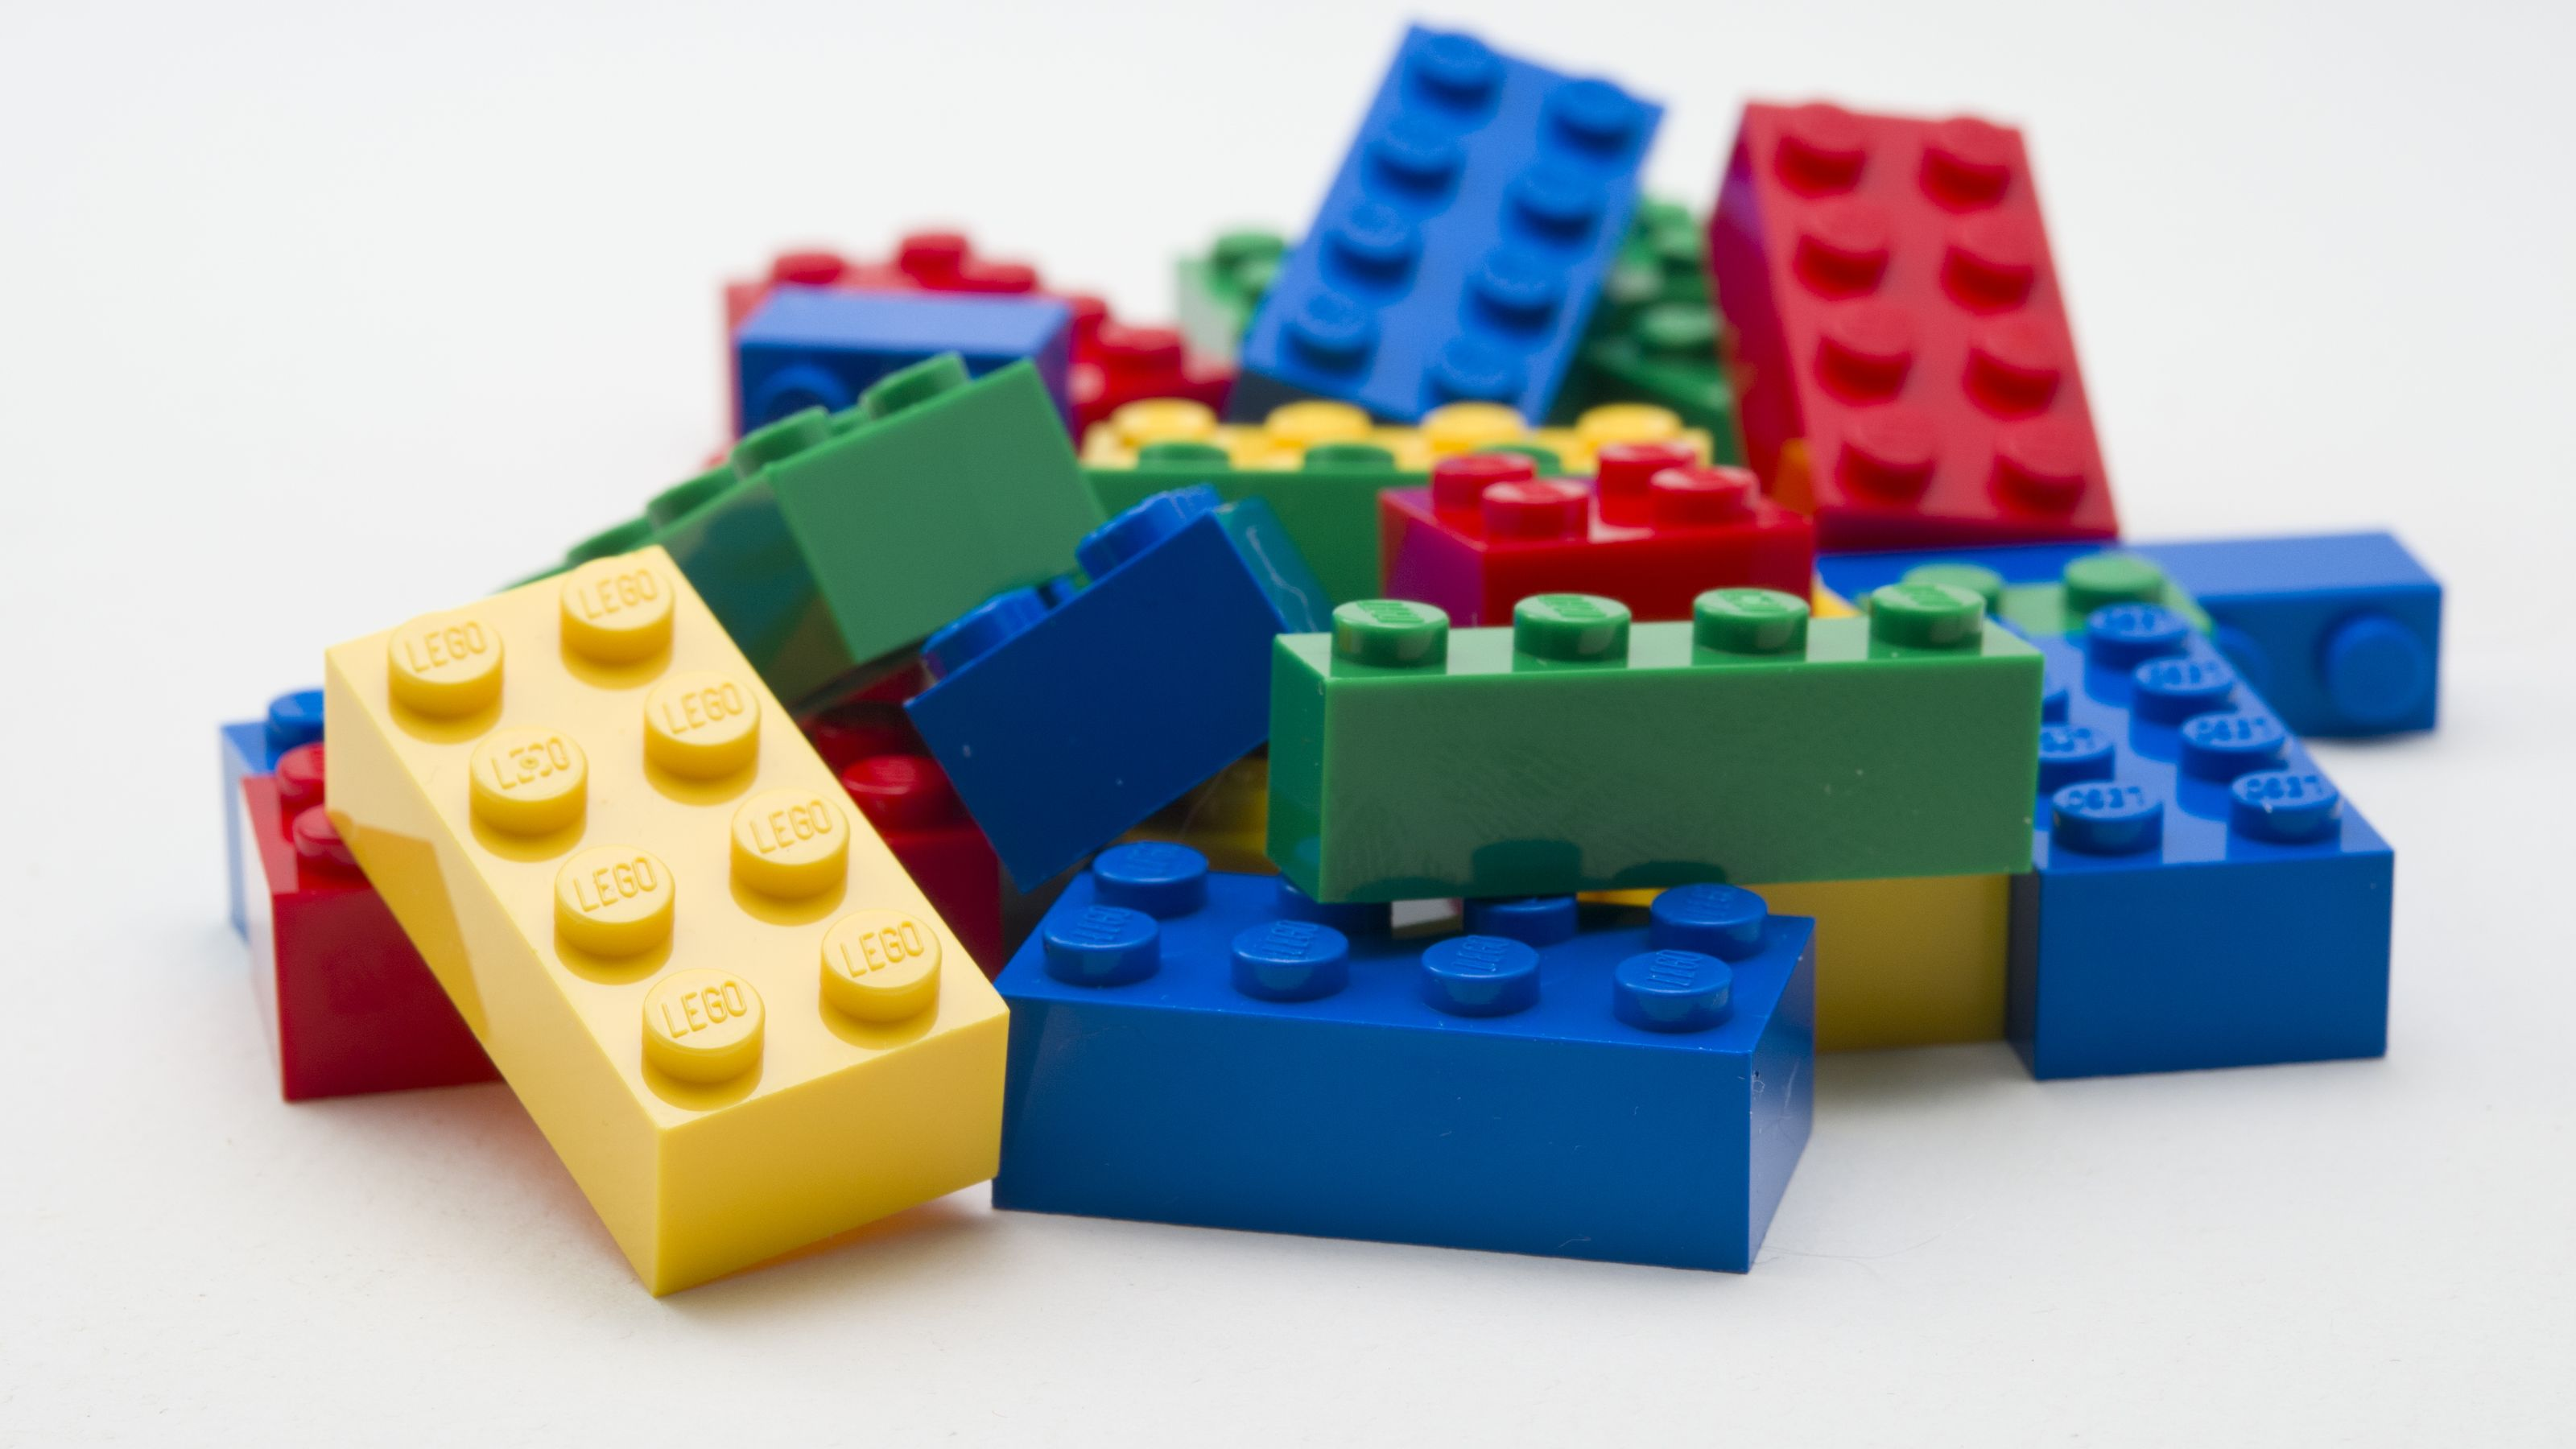
\includegraphics[width=7cm]{fig/lego.jpg}
     % \textit{``I believe I've isolated the algorithm for making friends.''}
     % \small{
     %   \hfill Sheldon Cooper, 
     %   \hfill in \textit{The Big Band Theory}, Season 2, Episode 13
%     }
    }
  \end{columns}
\end{frame}
 
%%%%%%%%%%%%%%%%%%%%%%%%%%%%%%%%%%%%%%%%%%%%%%%%%%%%%%%%%%%%%%%%%%%

\begin{frame}
  \frametitle{Construction d'un algorithme}
\begin{block}{Pour chaque probl�me, il vous est demand� de d�finir clairement :}
\begin{itemize}
\item Les �ventuelles \red{donn�es d'entr�e du probl�me} en pr�cisant leurs types et leur r�le,\\
\item les �ventuelles \red{donn�es de sortie du probl�me} en pr�cisant leurs types, \\
\item les diff�rentes \red{instructions} permettant d'obtenir les donn�es de sorties � partir
des donn�es d'entr�e.\\
\end{itemize}
\end{block}
\end{frame}

%%%%%%%%%%%%%%%%%%%%%%%%%%%%%%%%%%%%%%

\begin{frame}[fragile]
\frametitle{Exemple}
Algorithme qui d�termine le prix d'entr�e dans un mus�e (les mineurs payent moiti� prix)
\pause
\begin{columns}[t]
\column{6 cm}
\begin{exampleblock}{Donn�es}
\begin{algorithmic}[1]
\REQUIRE{age (entier)}\\
\COMMENT{age du client}
\ENSURE{tarif (d�cimal)}\\
\COMMENT{prix de l'entr�e}
\end{algorithmic}
\end{exampleblock}
\column{5 cm}
\pause

\begin{exampleblock}{Instructions}
\begin{algorithmic}[0]
\IF{age < 18}
\STATE tarif $\leftarrow$ 4
\ELSE
\STATE tarif $\leftarrow$ 8
\ENDIF
\RETURN{tarif}
\end{algorithmic}
\end{exampleblock}

\end{columns}
\end{frame}

%%%%%%%%%%%%%%%%%%%%%%%%%%%%%%%%%%%%%%%%%%%%%
\begin{frame}[fragile]
\frametitle{Structures conditionnelles 1/2}
\begin{columns}[t]
\column{6cm}
%\begin{block}

\begin{figure}
\begin{tikzpicture} [
    auto,
    decision/.style = { diamond, draw=blue, thick, fill=blue!20,
                        text width=1.5cm, text badly centered,
                        rounded corners, aspect=2 },
    block/.style    = { rectangle, draw=blue, thick, 
                        fill=blue!20, text width=1.5cm, text centered,
                        rounded corners, minimum height=2em },
    line/.style     = { draw, thick, ->, shorten >=2pt },
    node distance=1.5cm,
  ]
  \node (rac) {} ;
  \node (condition) [decision, below of=rac] {condition} ; 
  \node (center) [draw,circle,  thick, inner sep=2pt,minimum size= 0pt, radius = 2pt,below of =condition]{};
  \node (false) [block, left of=center,xshift=-3mm] {Action F};
  \node (true) [block, right of=center,xshift=3mm] {Action V};
   \node (end) [below of=center]{};
  % Define nodes in a matrix
  %\matrix [column sep=5mm, row sep=10mm] {
  %& \node (rac) {}; & \\
  %& \node [decision] (condition) {condition}; & \\
  %\node [block] (true) {Action V}; & & \node [block] (true) {Action V} ; \\
 % & \node (end) {}; \\
  %};
  
  % connect nodes
  \begin{scope}[every path/.style=line]
  \path (rac) -- (condition);
  \path (condition) -| node [near start, above] {vraie} (true);
  \path (condition) -| node [near start, above] {fausse} (false);
  \path (center) -- (end) ;
  %\path (false) -| (end);
  \end{scope}
  \draw[-, thick] (true) -- (center) ;
    \draw[-, thick] (false) -- (center) ;

\end{tikzpicture}
\end{figure}
%\end{block}
\column{5cm}

\begin{block}{}
\begin{algorithmic}[0]
\IF{\red{condition}}
\STATE Action V
\ELSE
\STATE Action F
\ENDIF
\end{algorithmic}
\end{block}

\begin{exampleblock}{Un exemple}
\begin{algorithmic}[0]
\IF{age < 18}
\STATE tarif $\leftarrow$ 4
\ELSE
\STATE tarif $\leftarrow$ 8
\ENDIF
\end{algorithmic}
\end{exampleblock}

\end{columns}
\end{frame}

\end{document}

%%%%%%%%%%%%%%%%%%%%% SECTION 1
\section{Les algorithmes}\label{section:1}
\begin{frame}
\begin{columns}
        \column{4.8cm}
            \tableofcontents[currentsection]
        \column{7cm}
        \centering{
            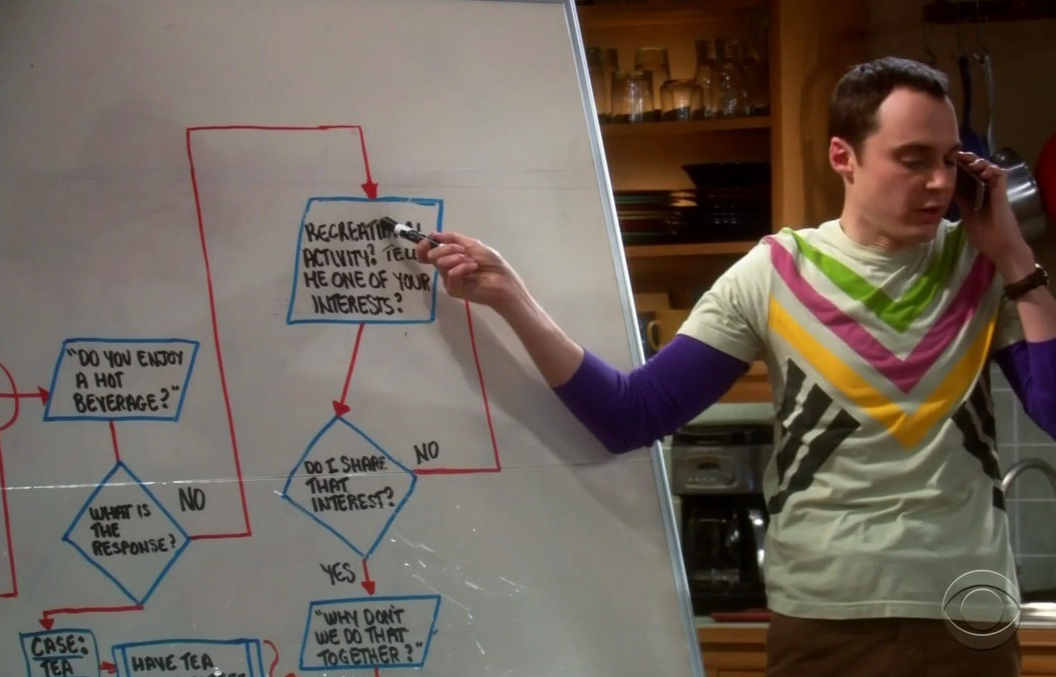
\includegraphics[width=7cm]{fig/Algorithm-sheldon.png}
            
                 \textit{ I believe I've isolateblblblblblblsblbslbslbsl
            sblbslblsblsblblsblbs
            lbslblbslsb d the algorithm for making friends.}
     
            
            \small{
            \hfill Sheldon Cooper, 
            
            \hfill in \textit{The Big Band Theory}, Season 2, Episode 13
            }
}

    \end{columns}

\end{frame}


%%%%%%%%%%%%%%%%%%%%%
\subsection{Introduction}
    \begin{frame}
    \frametitle{Pourquoi faire appel � des algorithmes ?}
    Pour automatiser des t�ches
    
    Exemples :
    \begin{itemize}
    \item M�tier � tisser\\
    \item M�thode de calcul � la main d'une division\\
    \item Recette de cuisine\\
    \item ...\\
    \end{itemize}
    \end{frame}
 
 %%%%%%%%%%%%%%%%%
 
    \begin{frame}
    \frametitle{Qu'est-ce qu'un algorithme ?}
    \begin{block}{D�finition}
    Un algorithme est un ensemble 
    ordonn� d'instructions simples
permettant de r�soudre un probl�me.
    \end{block}
    \end{frame}
    
 %%%%%%%%%%%%%%%%%%
 \subsection{Construction d'un algorithme}
%%%%%%%%%%%%%%%%%%%    
\section{La machine de Turing}
%%%%%%%%%%%%%%%%%%%%
 
  
\begin{frame}[fragile]
\frametitle{Un peu d'histoire...}
\begin{codeblock}{Test}
\begin{codeC}
for (int i = 0 ; i < n ; i ++) {
    //a comment
    printf("%d",i);
    }
\end{codeC}
\end{codeblock}

\begin{termblock}{test 2}
\lstset{escapeinside={��}}
\begin{lstlisting}
�\textbf{>>}�./a.out
�\color{darkgray}{\texttt{  Hello World}}�
\end{lstlisting}
\end{termblock}

 \begin{block}{Bloc standard}
blablabla
\end{block}
\end{frame}

\end{document}
